% Source - https://tex.stackexchange.com/a/758425
% Posted by egreg
% Retrieved 2026-01-18, License - CC BY-SA 4.0

\documentclass[tikz,border=5pt]{standalone}
\usetikzlibrary{decorations.pathreplacing}

\ExplSyntaxOn
\NewDocumentCommand{\Aterm}{m}{\__explorer_aterm:n {#1}}
\NewDocumentCommand{\Bterm}{mm}{\__explorer_bterm:nn {#1}{#2}}

\cs_new_protected:Nn \__explorer_aterm:n
 {% #1 = final index
  a \sb {1}
  \int_step_inline:nnn {2} {#1} { + a \sb {##1} }
 }
\cs_new_protected:Nn \__explorer_bterm:nn
 {% #1 = index, #2 = final index
  b \sb {#1}
  \int_compare:nT { #1<#2 } { - b \sb { \int_eval:n {#1+1} } }
 }
\ExplSyntaxOff

\begin{document}

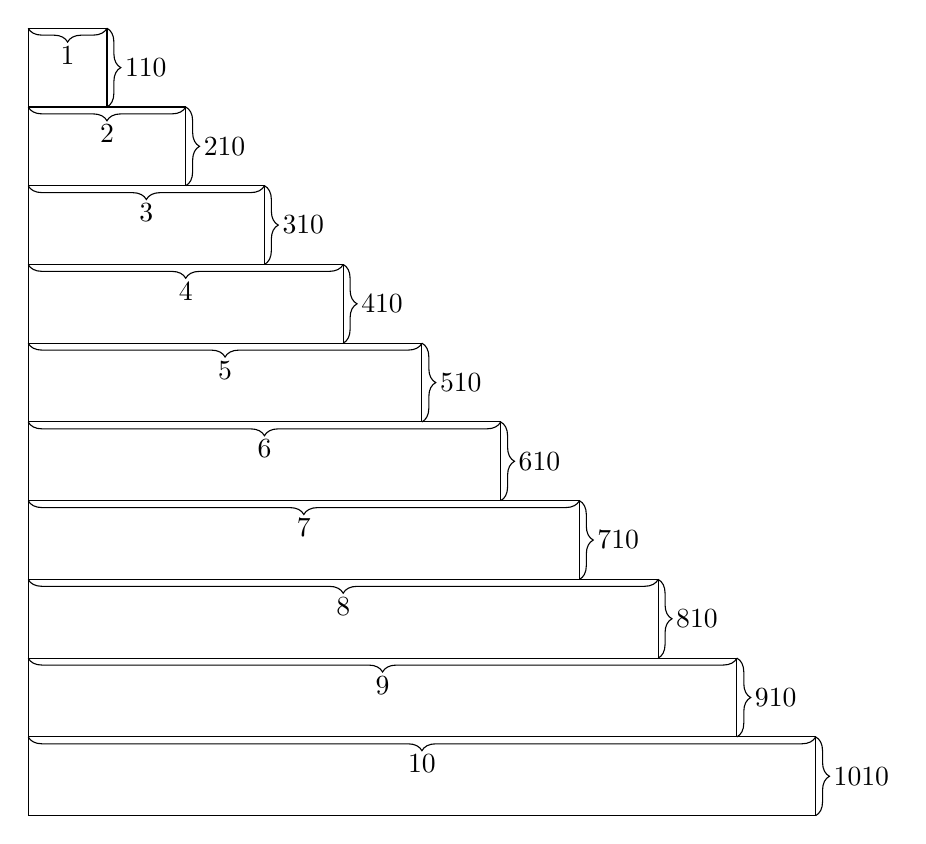
\begin{tikzpicture}[
  mybrace/.style={decorate,decoration={brace,amplitude=5pt,#1}},
]
  \def\NN{10}
  \foreach \i in {1,...,\NN}{
    \draw (0,{-(\i-1)}) rectangle (\i,-\i);
    \draw[mybrace] (\i,{-(\i-1)}) -- node[midway,right=3pt] {$\Bterm{\i}{\NN}$} (\i,-\i);
    \draw[mybrace=mirror] (0,{-(\i-1)}) -- node[midway,below=3pt] {$\Aterm{\i}$} (\i,{-(\i-1)});
  }
\end{tikzpicture}
\end{document}
